%workshopProposalTemplate.tex
\documentclass[12pt]{article}
\voffset=-1.4mm
\oddsidemargin=17pt \evensidemargin=17pt
\headheight=9pt     \topmargin=26pt
\textheight=576pt   \textwidth=440.8pt
\parskip=0pt plus 3.1pt
\raggedbottom
\usepackage{enumerate}
\usepackage[final]{pdfpages} 

\begin{document}

\title{\vspace{-4ex}Towards a unified workflow for multi contact motion on legged robots: Challenges in planning, optimization and control.}
%~ \author{Organizers:
	%~ Name 1,
	%~ Name 2,
	%~ Name 3\\
	%~ Directorate Liaison: Name of Liaison}
%~ \date{Dates in 20??, at SAMSI}
\maketitle

%~ \noindent
%~ A proposal for a SAMSI workshop should contain the following items.

\section{\textbf{Title} of proposed workshop}
Towards an unified workflow for multi contact motion or legged robots: Challenges in planning, optimization and control.

\section{Duration of the workshop}
Full-Day Workshop.

\section{Organizers}
Steve Tonneau: primary contact person \\
\textbf{affiliation}: Post doctorate researcher at LAAS-CNRS, Gepetto team.\\
\textbf{address}: 7 avenue du Colonel Roche, 31400 Toulouse\\
\textbf{phone}: (+33) 5-61-33-68-90\\
\textbf{email}: stonneau@laas.fr
\textbf{url}: http://stevetonneau.fr\\ \\
Timothy Bretl \\
\textbf{affiliation}: Associate Professor of Aerospace Engineering, University of Illinois\\
\textbf{address}: 148 Coordinated Science Laboratory, MC-228, 1308 West Main Street, Urbana, IL, 61801-2307, USA \\
\textbf{phone}: 217-244-3126 \\
\textbf{email}: tbretl@illinois.edu 
\textbf{url}: http://bretl.csl.illinois.edu\\ \\
Nicolas Mansard \\
\textbf{affiliation}: Permanent researcher at LAAS-CNRS, Gepetto team.\\
\textbf{address}: 7 avenue du Colonel Roche, 31400 Toulouse\\
\textbf{phone}: (+33) 5-61-33-68-90\\
\textbf{email}: nicolas.mansard@laas.fr
\textbf{url}: http://homepages.laas.fr/nmansard\\ \\
Igor Mordatch\\
\textbf{affiliation}: Graduate student at the University of Washington.\\
\textbf{address}: 185 Stevens Way, Room 370 Seattle, WA 98195\\
\textbf{phone}: (+1) 510 459 3152\\
\textbf{email}: mordatch@cs.washington.edu
\textbf{url}: http://homes.cs.washington.edu/~mordatch\\


\section{Website url}
http://homepages.laas.fr/nmansard/entracte/index.php?n=Publication.WorkshopIcra2015

\section{\textbf{Abstract}}
Early contributions on multi contact locomotion for legged robots have underlined the complexity of planning and executing motions in cluttered environments. In both the robotics and computer-graphics community, a large variety of approaches have been recently proposed to tackle the problem, thus often targeting one specific aspect: the planning of a feasible path for the robot, the optimization of its trajectory, or the feedback control of the robot during
the execution of a dynamic motion. Integrating these different aspects is not only an engineering issue. It raises scientific questions in terms of robustness of the algorithms and performance requirements. The objective of this workshop is to gather people working in these fields and propose a debate on the combination of these various aspects into a functional workflow for robot motions in cluttered environments.
Renowned speakers from the robotics and computer graphics field will present their work, and recommend the reading of selected papers prior the conference.  This will provide the audience with the ability to prepare their venue and ask relevant questions that will be analyzed by student groups and discussed during dedicated debate sessions.


\section{Content}
\subsection{Situation of the problem}
Achieving multi-contact locomotion is challenging: Theoretically, the motion or manipulation planning problem is known to be particularly difficult due to the complex topology of the configuration space. In practice, the execution of a planned trajectory on a robot requires the resolution of the problem of moving in contact while maintaining the balance of an underactuated unstable system. 

This problem is recognized by both the robotics and computer-graphics community, and their respective approaches have a lot to share.
It has gained visibility and interest with the advent of humanoid and legged robots, and in particular with the DARPA Robotics Challenge. While impressive advances have been emphasized, the challenge also shown that legged robots are far to be as mature as wheeled robots.

The problem can be roughly divided in three aspects. At the planning level, it is often considered to compute a discrete sequence of statically balanced key contact postures. In a second level, the complete continuous trajectory connecting all the postures is considered. The last level considers the control law that executes the complete movement on the robot despite the uncertainties of the model. These three aspects of the problem are strongly correlated and might be treated separately to reduce the complexity or together to provide a better approximation of a targeted optimality.

\subsection{Objective}
The workshop aims at gathering the key researchers studying all the three aspects of the problem, to provide an exhaustive painting of the state of the art, the current blocking problems and the future promising directions. One originality is that we have brought several key researchers from the computer-graphics community to share their viewpoints with the roboticists.

\subsection{Organization of the day}
The workshop consists in three topic specific presentation sessions, completed by two inter topic debate/poster sessions. These sessions are organized in an original fashion so as to enhance exchange and communication: the talks of each session will be completed with a topic specific
debate session, prepared by students.
A few months before the workshop, each presenter will recommend the reading of one or two papers, available on the workshop website. 
The students will read the paper, collect questions asked online by the public, and prepare a critic presentation of the papers that will start the debate session. Additionally, the audience will be given the opportunity to ask questions in real time using social networks during presentations.

An inter topic poster session aims at connecting two topic specific research issues, namely motion planning / trajectory generation and trajectory generation / robot control, and will result from a call for poster contributions.

We propose the following planning tentative: \\

\textbf{08.30}: Welcoming and introduction

\textbf{08.40}: Motion planning: 3 talks + topic debate

\textbf{10.25}: Coffee break

\textbf{10.40}: Trajectory optimization: 3 talks + topic debate

\textbf{12.25}: Dinner break

\textbf{13.25}: Poster session 1

\textbf{14.25}: Robot feedback control: 3 talks + topic debate

\textbf{16.15}: Poster session 2

\textbf{17.15}: Conclusion and farewell
%~ 
%~ The topics covered are:
%~ \begin{itemize}
%~ \item Motion and contact planning in cluttered environments
%~ \item Generation of contact trajectories through optimization
%~ \item Feedback control for executing multi contact motions on actual robots
%~ \end{itemize}
%~ 
%~ The debate sessions aim at discussing the specific issue of connecting these three topics so as to obtain a fully functional workflow from the planning to the robot.
%~ 
%~ A presentation session covers a specific aspect of multi contact planning for robots and  consists in:
%~ A long review talk (35 min)
%~ 2 specific talks (15 min each)
%~ A topic specific debate session, animated by a group of students
%~ 
%~ The topic specific debate is prepared before the event by the students, according to an agenda:
%~ A few months before the workshop, each presenter will recommend the reading of one or two papers, available on the workshop website. 
%~ The students will read the paper, collect questions asked online by the public, and prepare a critic presentation of the papers that will start the topic specific debate session. 
%~ Additionally, the audience will be given the opportunity to ask questions in real time using social networks.
%~ 
%~ An inter topic poster session aims at connecting two topic specific research issues, namely motion planning / trajectory generation and trajectory generation / robot control. They will have the following form:
%~ A “fast forward” session, where the authors of poster will present a teaser of their poster in two minutes;
%~ The actual poster session, resulting from a call for contributions, will follow on these specific aspects.



\section{List of confirmed speakers}
Because of the time constraints of some of the invited speakers, we ask that the workshop happens on the second day. \\ \\
All the speakers have confirmed their presence, although not all of them have been able to provide us with the title and / or abstract
of their presentation. \\ \\
\textbf{Speaker}: Russ Tedrake, MIT, USA \\
\textbf{Title}:  Robust feedback stabilization through unscheduled contact.\\
\textbf{Abstract}:  \\ \\
\textbf{Speaker}: Antonio Bicchi, University of Pisa, Italy (Unconfirmed)\\
\textbf{Title}: \\
\textbf{Abstract}: \\ \\
\textbf{Speaker}: Karen C. Liu, Georgia Tech University, USA \\
\textbf{Title}:  \\
\textbf{Abstract}:  \\ \\
\textbf{Speaker}: Shunichi Nozawa, The university of Tokyo, Japan \\
\textbf{Title}:  Planning and execution of whole-body environment and object
manipulation with a life-sized humanoid robot \\
\textbf{Abstract}: In this presentation, we introduce planning and execution system for whole-body environment and object manipulation with a life-sized humanoid robot by adaptive selecting of manipulation strategy and robust motion execution through haptic sensing of actual contact states and object's motion. \\ \\
\textbf{Speaker}: Adrien Escande, CNRS/AIST, JRL, Tsukuba, Japan \\
\textbf{Title}:  \\ 
\textbf{Abstract}:  \\ \\
\textbf{Speaker}: Igor Mordatch, University of Washington, USA \\
\textbf{Title}:  \\
\textbf{Abstract}:  \\ \\
\textbf{Speaker}: Quang-Cuong Pham, Nanyang Technological University, Singapore \\
\textbf{Title}:  \\
\textbf{Abstract}:  \\ \\
\textbf{Speaker}: Steve Tonneau, LAAS CNRS, France \\
\textbf{Title}: Interactively planning truly feasible contact sequences for legged robots.\\
\textbf{Abstract}: Recent progress in multi contact planning hold the promise of interactively generating feasible plans for legged robots, executed on the fly.
However, existing multi contact planners do not sufficiently take into account the dynamic limitations of the robots for which the planning is performed, nor for the uncertainties of the environment. The sad truth is that in cluttered environments, executing a planned motion is at best extremely hard, at worst simply impossible. Introducing such
robustness into modern contact planners is thus a necessary condition for the design of a complete, unsupervised
motion synthesis framework that will truly provide legged robots with motion autonomy. I will
present the latest results obtained in the domain of robust contact planning, and discuss the most exciting perspectives
in this regard.\\ \\
\textbf{Speaker}: Siddhartha Srinivasa, Carnegie Mellon University \\ 
\textbf{Title}: Physics-based manipulation under clutter and uncertainty \\
\textbf{Abstract}: My research goal is to bridge the gap between what robots can do now and what they are capable of doing. Towards that goal, I will overview some of our recent work on (1) using physics to increase the repertoire of manipulation actions beyond pick-and-place to nonprehensile and whole-arm manipulation, (2) orchestrating this repertoire to reconfigure clutter, (3) using physics to funnel uncertainty via open-loop robust controllers, and (4) representing uncertainty via state estimators and reducing uncertainty via information-seeking actions. \\ \\

\section{Plan to solicit participation}
The recent popularity of research in Multi contact planning, illustrated by events such as the Darpa Challenge, goes beyond the field of robotics, with collaborations in the computer graphics community. In the last five years several papers have been the highlight of the highly renowned SIGGRAPH conference, and Karen Liu, author of several of them, is one of our key speakers. This will provide the workshop with a strong visibility in this community.

Similarly, the list of confirmed speakers include some of the most renowned researchers in robotics.
The workshop format is a unique chance for researchers, especially young students, to collaborate and exchange with the speakers.

Because it is multidisciplinary and aims at creating synergies between researchers from motion planning, optimization and control, and character animation for computer graphics, we expect an important attendance.

\section{Plan to encourage interaction among participants}
One originality of the workshop lies in the fact that prior to the conference, a reading list will be given online, allowing people to prepare and submit their questions in advance. This aspect was appreciated by invited speakers such as Russ Tedrake, and we believe that the work produced prior to the conference will encourage on site discussion.

The workshop is also organized in a way that allow speaking time to established researchers, but also young students which will have prepared their interventions and be less intimidated to speak in public.

Furthermore, during the presentations the audience will be given the opportunity to ask questions online using twitter or the conference website. These questions will be in turn asked by the organizers during he dedicated debate sessions.

\section{Equipments}
In addition to standard equipment we
anticipate the need of a number of 20 poster interactive screens
or stands.

\section{Support of an IEEE RAS Technical Committee}
The workshop is supported by the Whole Body Control Technical Commitee, represented by Dr. Luis Sentis.
It is also supported by Prof. Dr. Katja Mombaur, chair of the Technical Comitee on Model-based Optimization.

\section{Attachements}
Attached to this proposal are:
\begin{itemize}
\item The letters of support from the Whole Body Control and Model-based Optimization TC;
\item The history of email exchange with the confirmed speakers, proving that they accepted to talk.
The relevant parts of these long logs are underlined. The two remaining speakers, Steve Tonneau and Igor Mordatch,
are members of the organization.
\end{itemize}

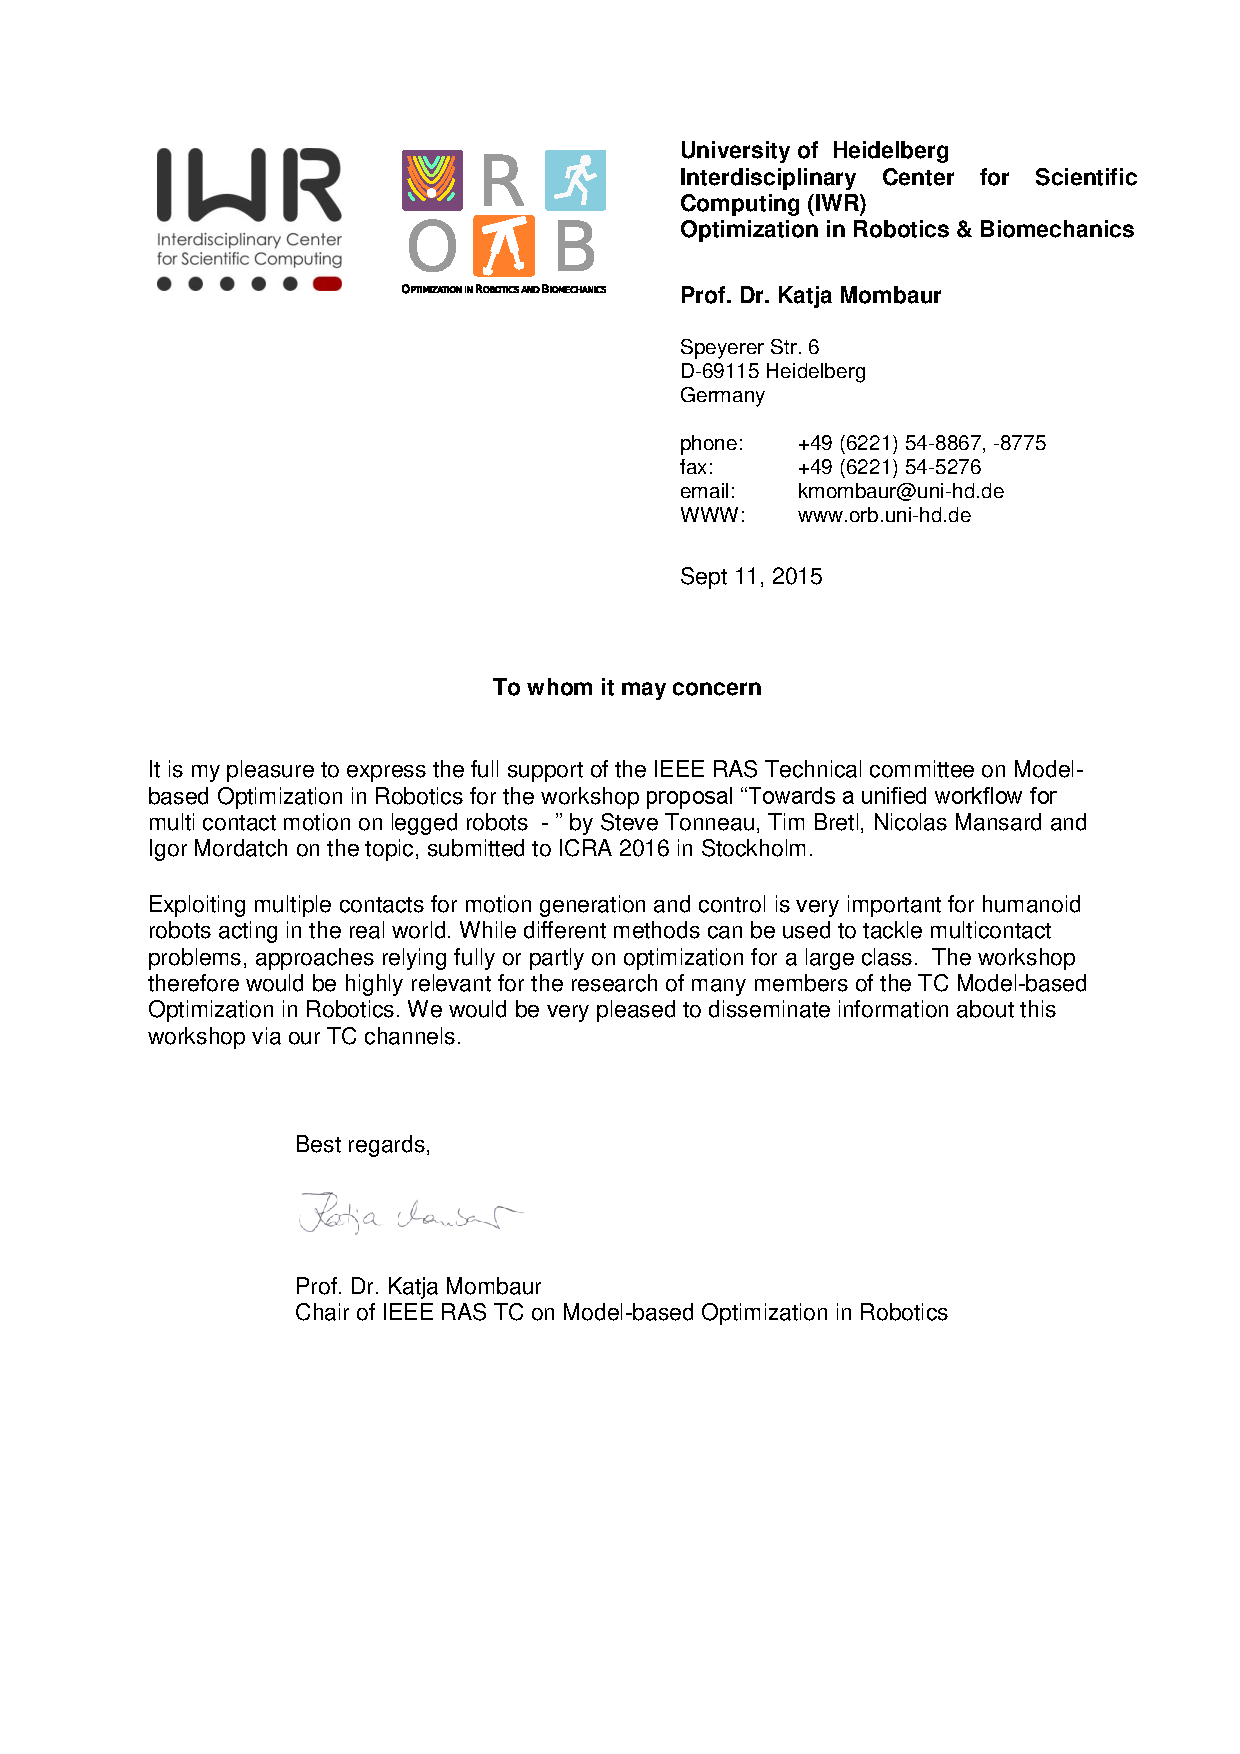
\includepdf[pages=1]{support_icra2016_nicolas.pdf}
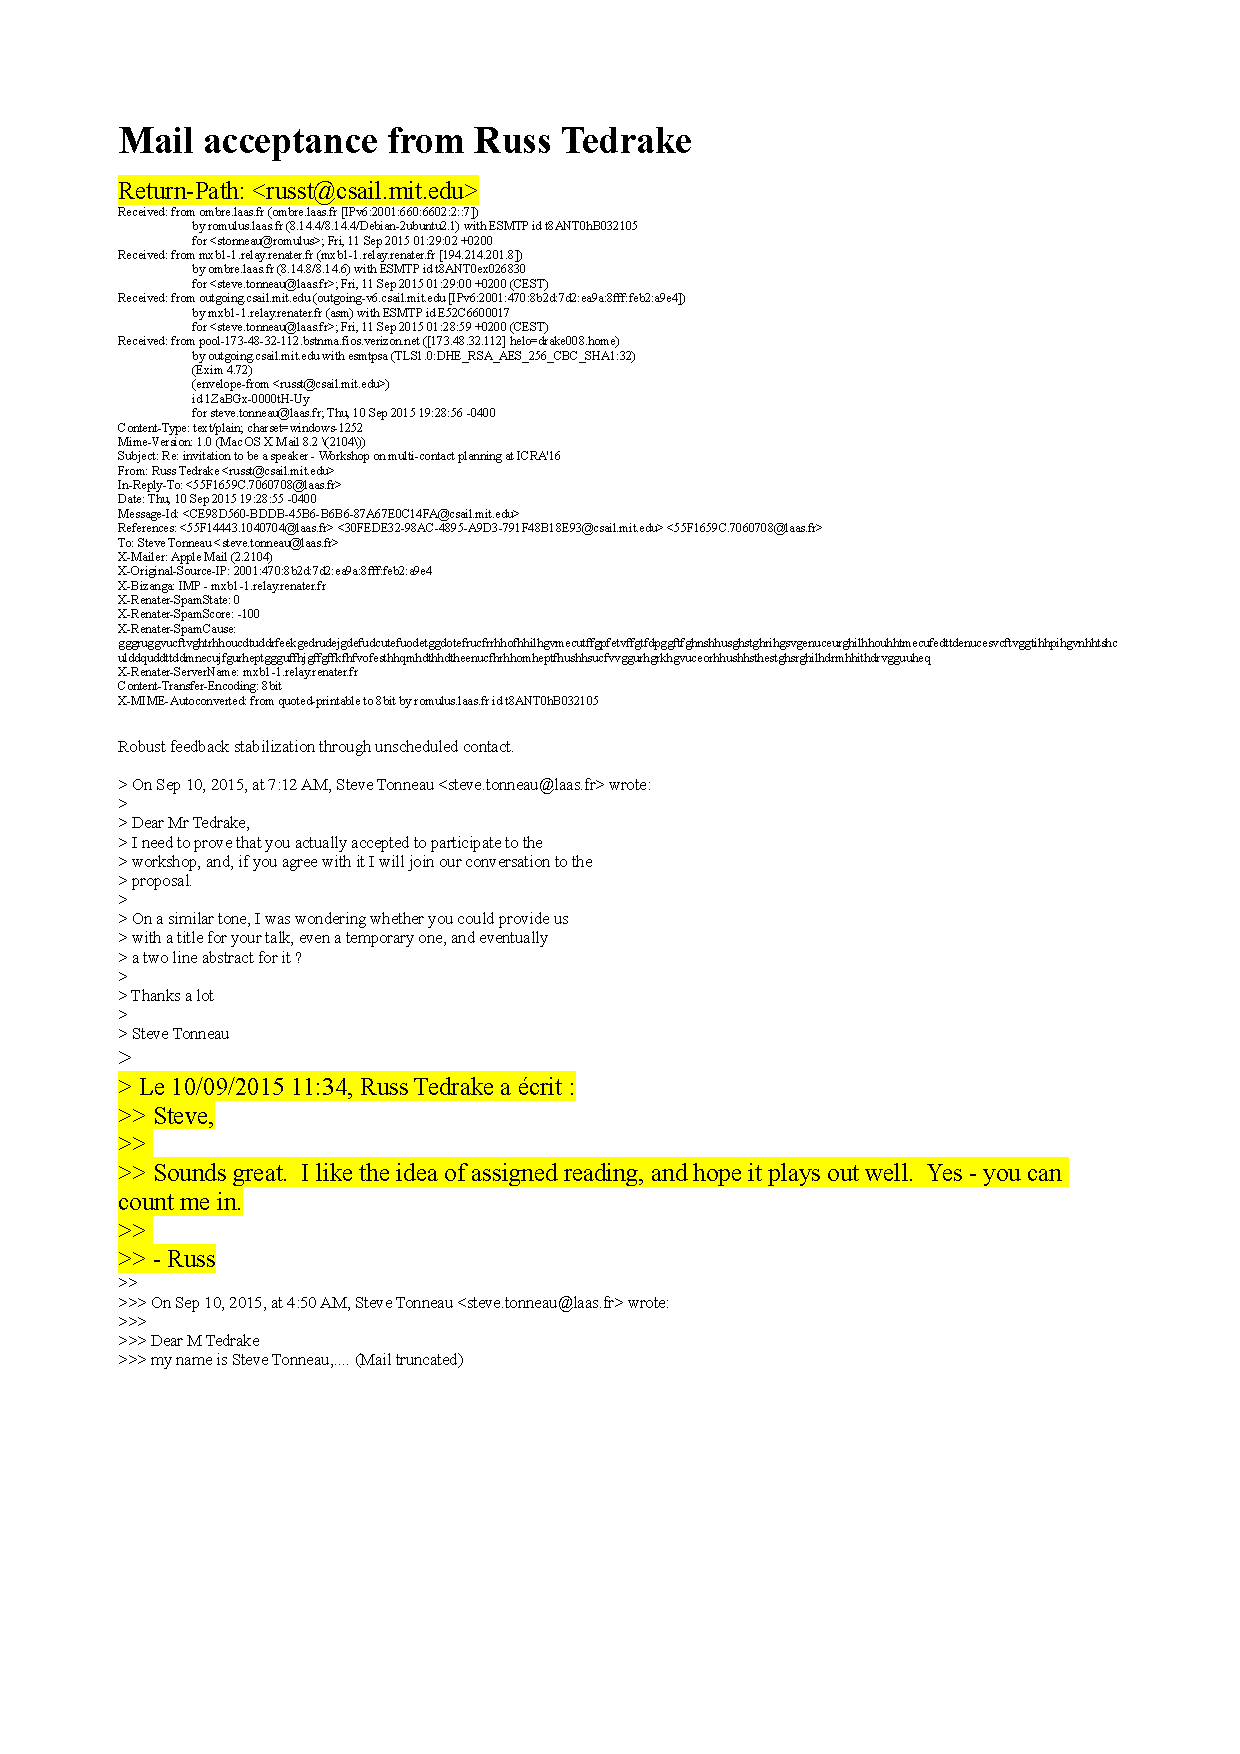
\includepdf[pages=1]{mails.pdf}
\includepdf[pages=2]{mails.pdf}
\includepdf[pages=3]{mails.pdf}
\includepdf[pages=4]{mails.pdf}
\includepdf[pages=5]{mails.pdf}
\includepdf[pages=6]{mails.pdf}

\end{document}
